\documentclass[11pt,a4paper]{article}
\usepackage[utf8]{inputenc}
\usepackage[T1]{fontenc}
\usepackage[spanish]{babel}
\usepackage[margin=2.5cm]{geometry}
\usepackage{amsmath, amssymb}
\usepackage{graphicx}
\usepackage{xcolor}
\usepackage{caption}
\usepackage{booktabs}
\usepackage[hidelinks]{hyperref}
\usepackage{titlesec}

% Section styling similar to the previous document
\titleformat{\section}{\normalfont\Large\bfseries\color{blue!50!black}}{\thesection}{1em}{}
\titleformat{\subsection}{\normalfont\large\bfseries\color{blue!50!black}}{\thesubsection}{1em}{}

\setlength{\parskip}{0.5em}
\setlength{\parindent}{0pt}

\title{\textbf{Contribución de la rugosidad de interfaz al defasaje en QCLs THz fríos}\\[0.3em]
\large Un cálculo de una etapa activa de tres pozos, sin parámetros ajustados a $T_2$}
\author{Vladyslav Savytskyy}
\date{Mayo 2026 \quad --- \quad Argentina}

\begin{document}
\maketitle

\begin{center}
\textit{Nota preliminar para discusión. Pensada para leerse antes de nuestra reunión.}
\end{center}

\vspace{1em}

\begin{abstract}
\noindent Este documento estima la contribución de la rugosidad de interfaz al
defasaje puro $\gamma_{\mathrm{pure}}$ del par de estados láser de una etapa
activa de tres pozos del tipo \emph{direct-phonon} a baja temperatura, usando
el modelo estándar de Ando con valores de literatura para los parámetros de
rugosidad ($\Delta = 0{,}2825$~nm, $\Lambda = 5$~nm). El cálculo no contiene
ningún parámetro ajustado al $T_2$ experimental. El resultado total,
$\gamma_{\mathrm{pure}}^{\,\mathrm{rug}} \approx 0{,}18~\mathrm{ps}^{-1}$,
es aproximadamente \emph{un cuarto} del valor experimental observado en QCLs
THz fríos ($\gamma_{\mathrm{pure}}^{\,\mathrm{exp}} \approx 0{,}65$--$1{,}0~\mathrm{ps}^{-1}$).
Dos interfaces del período concentran $\sim\!75\%$ de esa contribución. Esta
nota es deliberadamente modesta: identifica qué parte del presupuesto de
coherencia puede atribuirse a un mecanismo bien definido, y deja explícito
qué queda sin explicar.
\end{abstract}

\section{Por qué este cálculo}

En el modelado de QCLs THz el tiempo de defasaje $T_2$ suele aparecer como
parámetro fenomenológico que se ajusta a posteriori. El motivo es práctico:
$T_2$ recibe contribuciones de varios mecanismos a la vez (rugosidad de
interfaz, desorden de aleación, scattering de impurezas, fonones LO no
térmicos), y cada uno depende de detalles microscópicos que no es trivial
calcular por separado. Sin embargo, hay un mecanismo --- el más geométrico
de todos --- para el cual sí se puede dar un número defendible sin
\emph{ningún} ajuste posterior: la rugosidad de interfaz entre el pozo y la
barrera.

La pregunta operativa, entonces, es: \emph{¿cuánto del} $\gamma_{\mathrm{pure}}$
\emph{observado se explica solamente por la rugosidad de interfaz, calculada
con parámetros de literatura?} Si la respuesta es ``casi todo'', el resto del
modelado se simplifica enormemente. Si la respuesta es ``sólo una fracción'',
entonces se identifica cuantitativamente cuánto presupuesto queda para los
otros mecanismos, y se sabe dónde mirar.

Esta nota responde a esa pregunta para una etapa activa concreta. La respuesta
es ``una fracción, aproximadamente un cuarto'', y la mayor parte de esa
fracción está localizada en dos interfaces específicas del período.

\section{El modelo}

\paragraph{Geometría.} Una etapa activa biaseada de tres pozos en el sistema
GaAs / Al$_{0{,}15}$Ga$_{0{,}85}$As, con secuencia de capas (en nm):
\[
\underbrace{4{,}3}_{\text{barrera de inyección}} \,\big/\,
\underbrace{8{,}5}_{\text{pozo}_1} \,\big/\,
\underbrace{2{,}4}_{\text{barrera}} \,\big/\,
\underbrace{8{,}5}_{\text{pozo}_2} \,\big/\,
\underbrace{4{,}1}_{\text{barrera}} \,\big/\,
\underbrace{16{,}1}_{\text{pozo}_3 \text{ (inyector)}} \,\big/\,
\underbrace{4{,}3}_{\text{barrera}}.
\]
Composición de barrera $x = 0{,}15$ ($\Delta E_c = 135$~meV), bias aplicado
$F = 11$~kV/cm, masa efectiva $m^\star = 0{,}067\,m_e$. La geometría es
representativa de los diseños \emph{direct-phonon} reportados por Khalatpour
y colaboradores~\cite{khalatpour2021,khalatpour2024}.

\paragraph{Estados.} Diagonalización numérica de la ecuación de envolvente 1D
en una grilla de $0{,}05$~nm. Se identifican los dos estados cuyo solapamiento
con la región del par activo (pozos 1 y 2) es máximo y cuya separación cae en
la banda THz. En este diseño la separación resulta $E_{\mathrm{ULS}} -
E_{\mathrm{LLS}} = 19{,}3$~meV ($f = 4{,}67$~THz), un poco más alta que el
$\sim\!3{,}4$~THz típico de Khalatpour; la elección de capas se podría
refinar, pero la física que se discute no depende de eso.

\paragraph{Defasaje por rugosidad.} En el modelo de Ando, con
autocorrelación Gaussiana de la rugosidad
$\langle\eta(\mathbf{r})\eta(\mathbf{r}')\rangle = \Delta^2 \exp(-|\mathbf{r}-\mathbf{r}'|^2/\Lambda^2)$,
la contribución elástica intra-subbanda al defasaje puro de la coherencia
$|\mathrm{ULS}\rangle\langle\mathrm{LLS}|$ es~\cite{unuma2003,khurgin2008}:
\begin{equation}
\gamma_{\mathrm{pure}}^{\,\mathrm{rug}}
= \frac{m^\star\,\Delta E_c^{\,2}\,\pi\,\Delta^{2}\,\Lambda^{2}}{2\hbar^{3}}\;
\sum_{i}\bigl[\,|\psi_{\mathrm{U}}(z_i)|^{2}-|\psi_{\mathrm{L}}(z_i)|^{2}\,\bigr]^{2}\,F(k\Lambda),
\label{eq:gamma_pure}
\end{equation}
donde la suma corre sobre las interfaces del período, $F(k\Lambda) = \langle
\exp(-q^{2}\Lambda^{2}/4)\rangle_{\theta}$ es el factor angular promediado, y
los valores aceptados de literatura para GaAs/AlGaAs por MBE son
$\Delta = 0{,}2825$~nm (un monocapa) y $\Lambda \approx 4$--$6$~nm.

Conviene enfatizar lo que esta fórmula \emph{no} requiere: ningún ajuste a
$T_2$. Los inputs son $m^\star$, $\Delta E_c$, $\Delta$ y $\Lambda$, todos
con valores que existen en la literatura desde hace décadas y que no se
modifican aquí.

\section{Resultados}

\begin{figure}[h]
\centering
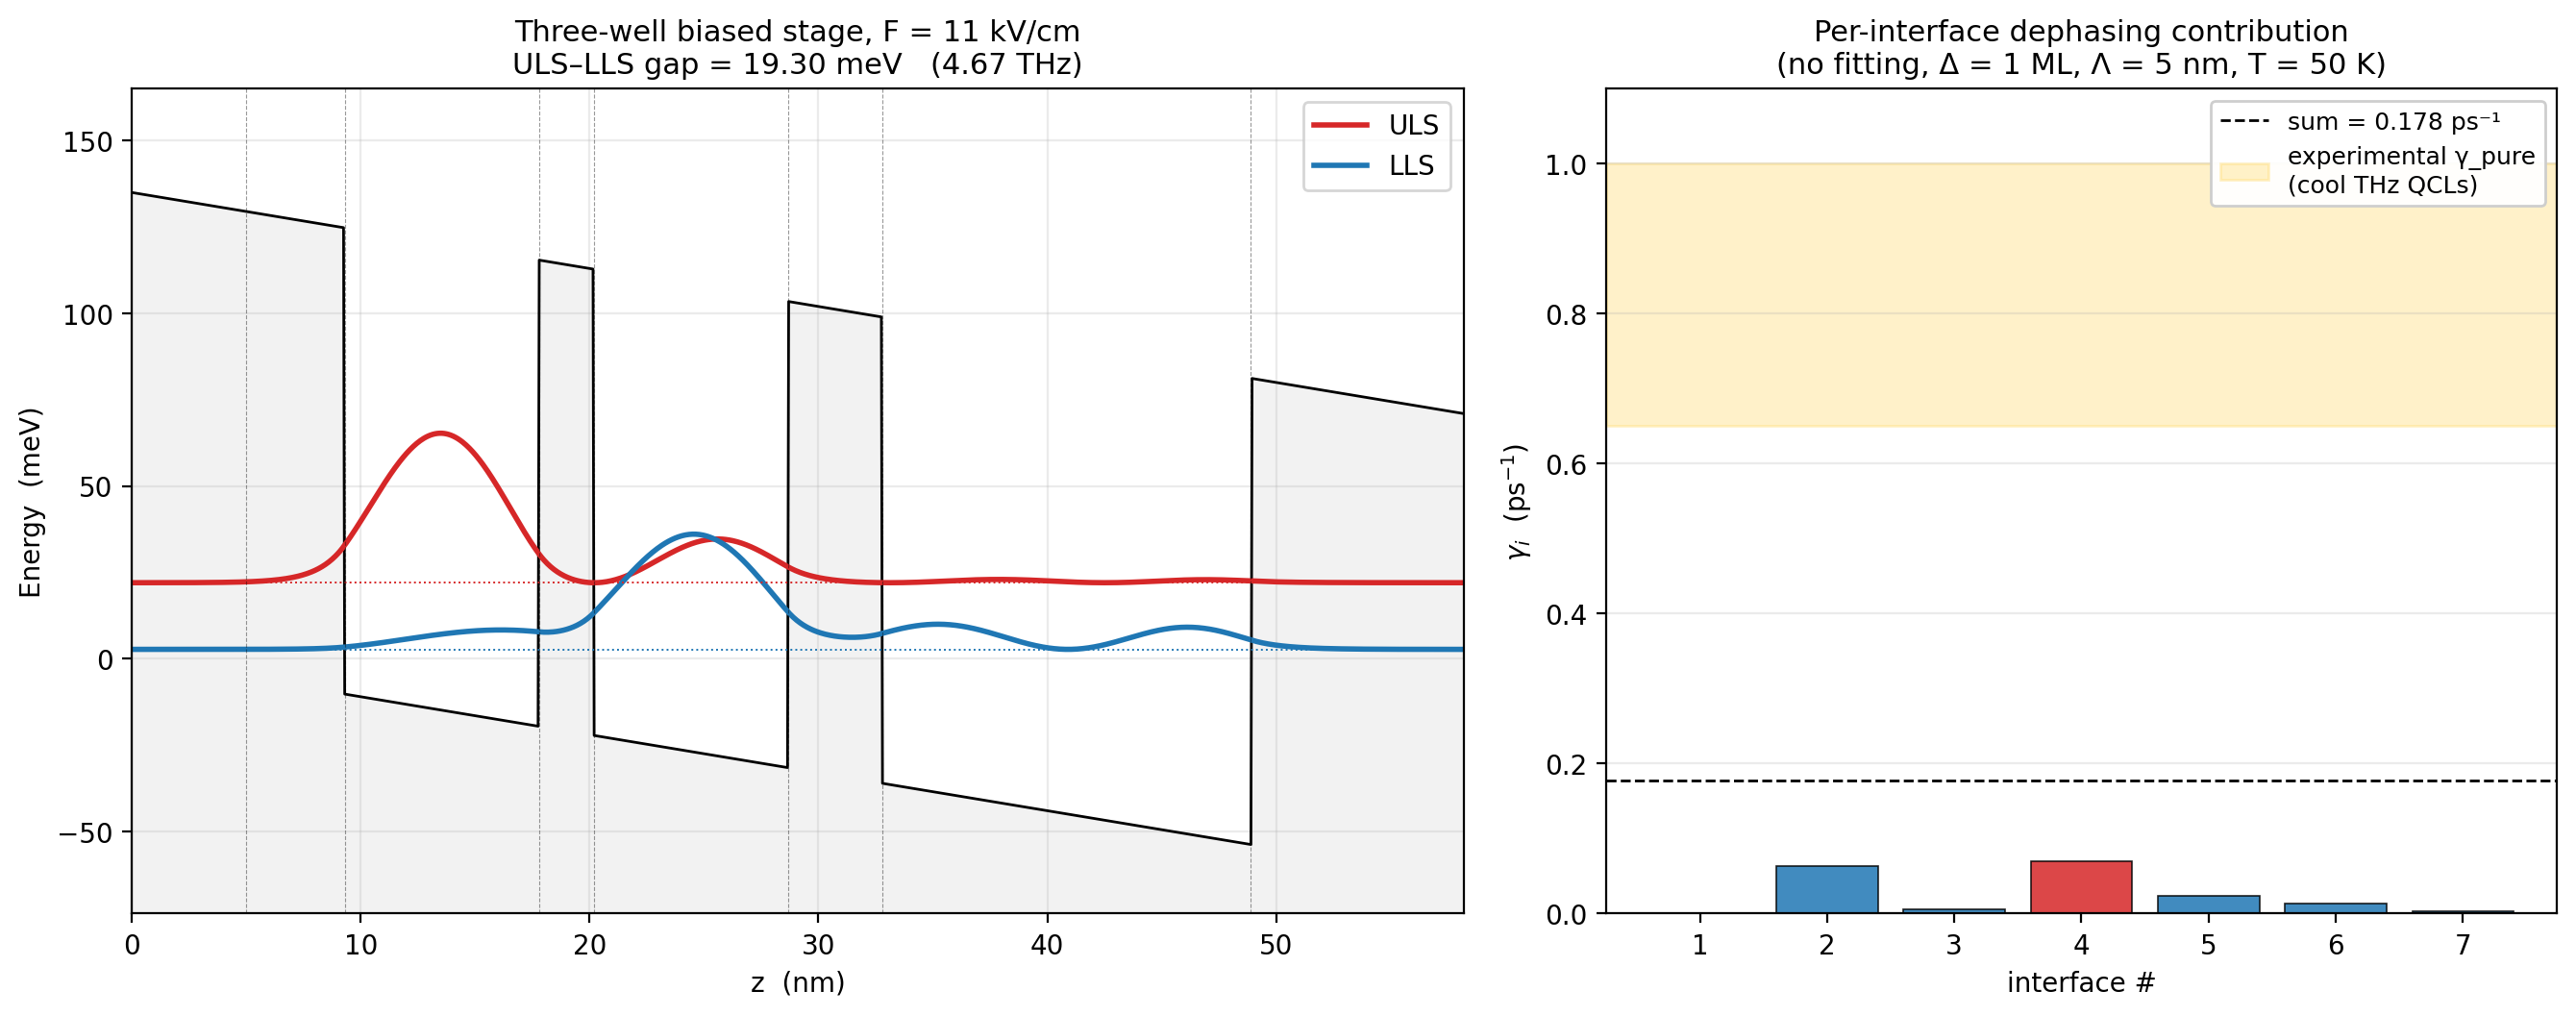
\includegraphics[width=\textwidth]{thz_threewell_dephasing.png}
\caption{\emph{Izquierda:} potencial de la etapa activa biaseada y densidades
de probabilidad de los estados láser superior (ULS, rojo) y láser inferior
(LLS, azul). \emph{Derecha:} contribución por interfaz a
$\gamma_{\mathrm{pure}}^{\,\mathrm{rug}}$, calculada con la ec.~\eqref{eq:gamma_pure}
usando $\Delta = 0{,}2825$~nm, $\Lambda = 5$~nm, $T = 50$~K. La línea
punteada negra indica la suma sobre las siete interfaces del período. La
banda amarilla indica el valor experimental de $\gamma_{\mathrm{pure}}$ en
QCLs THz fríos. La interfaz~4 (rojo, dominante) es el borde derecho del
pozo del LLS.}
\label{fig:main}
\end{figure}

La contribución total de la rugosidad, sumada sobre las siete interfaces
del período, da
\begin{equation}
\gamma_{\mathrm{pure}}^{\,\mathrm{rug}} \;=\; 0{,}178~\mathrm{ps}^{-1},
\qquad T_2^{*,\mathrm{rug}} \;=\; 5{,}6~\mathrm{ps}.
\label{eq:total}
\end{equation}
Comparado con el valor experimental $\gamma_{\mathrm{pure}}^{\,\mathrm{exp}}
\approx 0{,}65$--$1{,}0~\mathrm{ps}^{-1}$ (correspondiente a $T_2 \approx 1{,}0$--$1{,}5$~ps),
la rugosidad da cuenta de aproximadamente \textbf{20--25\,\%} del defasaje
observado.

La estructura por interfaz es informativa por sí sola
(Fig.~\ref{fig:main}, panel derecho):
\begin{itemize}
  \item Las interfaces 2 y 4 --- los bordes de los pozos del ULS y del LLS
        respectivamente --- aportan $\sim\!0{,}064$ y $\sim\!0{,}069~\mathrm{ps}^{-1}$,
        es decir un $\sim\!75\,\%$ del total.
  \item Las interfaces de la barrera delgada interior (3) y del pozo
        inyector (5--7) aportan en conjunto un $\sim\!25\,\%$.
  \item La interfaz~1 (cierre exterior de la barrera de inyección, hacia
        el período anterior) no contribuye: ahí ni el ULS ni el LLS tienen
        peso apreciable.
\end{itemize}

Esto es consistente con la intuición geométrica: el defasaje por rugosidad
está dominado por las interfaces donde $|\psi_\mathrm{U}|^2$ y $|\psi_\mathrm{L}|^2$
son más \emph{distintos} entre sí --- precisamente las interfaces que
flanquean los dos pozos principales del par activo.

\section{Discusión}

\subsection{El cuarto que sí está explicado}

La rugosidad de interfaz, con parámetros aceptados de literatura y sin
ningún ajuste a $T_2$, da $\sim\!0{,}18~\mathrm{ps}^{-1}$ de defasaje en
esta etapa. Esto es físicamente sólido y geométricamente localizado:
las dos interfaces inmediatamente alrededor del par activo cargan con
casi todo el presupuesto. Si en un diseño futuro se aumentara
artificialmente la rugosidad de esas dos interfaces (por ejemplo
introduciendo una interrupción de crecimiento), la predicción es que
$T_2$ degradaría aproximadamente como $\Delta^2 \Lambda^2$ proveniente
solo de esas dos interfaces.

\subsection{Los tres cuartos que no}

El resto, $\sim\!0{,}5$--$0{,}8~\mathrm{ps}^{-1}$, debe venir de otros
mecanismos no incluidos aquí. Los candidatos del tamaño correcto son:
\begin{itemize}
  \item \textbf{Desorden de aleación en las barreras de AlGaAs.} En este
        cálculo las barreras se tratan como potencial constante; el
        desorden composicional aleatorio en $x = 0{,}15$ contribuye a un
        defasaje elástico análogo al de la rugosidad, pero \emph{en volumen
        de barrera} en vez de en interfaz. Estimaciones razonables ubican
        esta contribución en el rango $0{,}2$--$0{,}5~\mathrm{ps}^{-1}$ para
        este tipo de diseño.
  \item \textbf{Fonones LO no térmicos.} A $T_\mathrm{lattice} = 50$~K la
        ocupación térmica de Bose para $\hbar\omega_\mathrm{LO} = 36$~meV
        es despreciable, pero la corriente inyecta fonones LO en
        no-equilibrio cuya distribución efectiva sí contribuye al
        defasaje. Esta es la contribución menos cuantificada en la
        literatura.
  \item \textbf{Scattering de impurezas ionizadas} en las regiones dopadas
        adyacentes (no incluidas en este modelo de un solo período).
\end{itemize}

Ninguno de estos tres mecanismos es ajustable libremente tampoco; cada uno
admite un cálculo del mismo estilo que el presentado aquí. Lo único que
falta es hacerlos.

\subsection{Una observación de diseño}

Si las interfaces 2 y 4 dominan el presupuesto de coherencia, entonces
\emph{la calidad de esas dos interfaces en particular} (no del crecimiento
en promedio) determina $\gamma_{\mathrm{pure}}^{\,\mathrm{rug}}$ del
dispositivo. Esto sugiere una pregunta operativa: ¿se observa
experimentalmente una correlación entre la calidad reportada de la barrera
central de $2{,}4$~nm (la más fina del período, y la que separa los dos
pozos del par activo) y el $T_2$ medido?

\section{Preguntas abiertas para la conversación}

Este documento es deliberadamente parcial. Las cosas sobre las cuales me
gustaría discutir cuando nos veamos:

\begin{enumerate}
\item ¿El número $0{,}18~\mathrm{ps}^{-1}$ es consistente con lo que vos
      observás --- en el sentido de que el resto del presupuesto ``cierra''
      con los otros mecanismos --- o resulta demasiado bajo?
\item ¿La localización en las dos interfaces internas se manifiesta en los
      datos cuando se varía el espesor de la barrera central, o el efecto
      queda enmascarado por otros canales?
\item ¿Hay literatura reciente que ataque el desorden de aleación en
      barreras AlGaAs con el mismo nivel de detalle (sin $T_2$ ajustado)?
      Lo que vi parece tratarlo siempre como contribución agregada.
\item ¿Tiene sentido extender este cálculo a varios bias para mapear cómo
      cambia la localización de $\psi_\mathrm{U}$ y $\psi_\mathrm{L}$ y
      cómo eso reasigna el peso entre interfaces? Esto podría dar una
      ventana operativa para optimización de diseño.
\end{enumerate}

Mi intención no es proponer un marco ni una predicción nueva. Es entregar
una pieza concreta del rompecabezas y preguntarte si encaja con lo que ves
desde tu lado.

\section{Sobre el código adjunto}

El cálculo está implementado en un único script Python \texttt{thz\_threewell.py}
(adjunto), de aproximadamente 200 líneas, que reproduce los números de la
ec.~\eqref{eq:total} y la Figura~\ref{fig:main} en menos de un minuto en
una máquina común. Requiere \texttt{numpy}, \texttt{scipy} y
\texttt{matplotlib} --- nada más. Para correrlo:

\begin{center}
\fbox{\parbox{0.85\textwidth}{\small
\texttt{\$ python3 thz\_threewell.py}\\[0.3em]
\textit{Salida: tabla por interfaz en stdout, más
\texttt{thz\_threewell\_dephasing.png} guardado en el mismo directorio que
el script.}
}}
\end{center}

Los parámetros de geometría (espesores de capa, bias, composición de
barrera) y los parámetros de rugosidad ($\Delta$, $\Lambda$) están todos al
principio del archivo, claramente marcados, para que sea trivial probar
variantes. Si querés cambiar a otra estructura o probar otra composición
$x$, son tres líneas.

\paragraph{Nota.} El código fue desarrollado con ayuda de un asistente de IA
(Claude, de Anthropic) en sesiones de revisión cruzada: yo planteaba las
preguntas físicas y verificaba los resultados, el asistente ayudó con la
implementación numérica y con detectar errores de signo y de unidades. La
responsabilidad de la elección del modelo, de la interpretación de los
resultados, y del contenido de este documento es mía.

\renewcommand{\refname}{Referencias}
\begin{thebibliography}{99}
\bibitem{unuma2003}
T.~Unuma, M.~Yoshita, T.~Noda, H.~Sakaki, H.~Akiyama,
\emph{Intersubband absorption linewidth in GaAs quantum wells due to scattering
by interface roughness, phonons, alloy disorder, and impurities},
J.~Appl.~Phys.\ \textbf{93}, 1586 (2003).

\bibitem{khurgin2008}
J.~B.~Khurgin,
\emph{Inhomogeneous origin of the interface roughness broadening of
intersubband transitions},
Appl.~Phys.~Lett.\ \textbf{93}, 091104 (2008).

\bibitem{khalatpour2021}
A.~Khalatpour, A.~K.~Paulsen, C.~Deimert, Z.~R.~Wasilewski, Q.~Hu,
\emph{High-power portable terahertz laser systems},
Nat.~Photonics \textbf{15}, 16 (2021).

\bibitem{khalatpour2024}
A.~Khalatpour \emph{et al.},
\emph{Enhanced operating temperature in terahertz quantum cascade lasers
based on direct phonon depopulation},
Nat.~Commun.\ (2024).

\bibitem{ando1982}
T.~Ando, A.~B.~Fowler, F.~Stern,
\emph{Electronic properties of two-dimensional systems},
Rev.~Mod.~Phys.\ \textbf{54}, 437 (1982).
\end{thebibliography}

\end{document}
